\restylefloat{table,figure}
\pagestyle{fancy}
\cfoot{\thepage}
\renewcommand{\footrulewidth}{0.25pt}


\section{Dati}
Gli ambiti più importanti nei quali vengono applicate tecniche di machine learning nella vita reale sono diversi, in particolare si usano in:
finanza, sanità, agricoltura, e-commerce, social, chatbot, sensoristica (come i veicoli a guida autonoma).

Vista la grande mole di dati la necessità è capire come trattare i dati.

\textbf{L'obiettivo del Machine Learning è sviluppare metodologia per dare valore ai dati in funzione di una particolare domanda che ci stiamo facendo.}

Tipicamente le tecninche di machine learning si dividono nelle seguenti tre macro categorie:
\begin{itemize}
	\item Apprendimento supervisionato o predittivo: qualcuno ha gia catalogato ad esempio delle immagini o dei dati e noi prendendo questi modelli dovremmo essere in grado di predire.
	\item Apprendimento descrittivo: ci sono delle funzioni obiettivo che vanno ottimizzate. Non usiamo etichette della singola istanza ma in qualche modo sappiamo dove arrivare.
	\item Apprendimento rinforzato: E' quello più utile in questa epoca: funziona sui premi.
\end{itemize}

In questo corso ci concentreremo sui primi due tipi di apprendimento.

L' \textit{apprendimento supervisionato} si divide a sua volta nelle seguenti due categorie:
\begin{itemize}
	\item Classificazione: quando il problema consiste nel dividere in classi delle quantità discrete.
	\item Regressione: quando il problema consiste nel ricostruire una certa variabile date delle condizioni pregresse.
\end{itemize}

L' \textit{apprendimento non supervisionato} si divide a sua volta in:
\begin{itemize}
	\item Clustering: Quando il problema consistere nel ricostruire delle classi delle istanze che ci vengono consegnate, senza sapere nulla sulla storia pregressa.
	\item Associativa: Quando il problema consiste nel scoprire pattern che descrivono bene caratteristiche associate ad un certo fenomeno.
\end{itemize}

Per alcuni compiti la correlazione statistica va benissimo, in alcuni casi però essa è addirittura deleteria.  Se infatti provassi a vedere la correlazione tra il numero di omicidi in america e il numero di fondi investiti sulla ricerca scientifica vedrei che statisticamente sono strettamente correlate. Questo è un no-sense ed è il classico esempio di \textit{correlazione spuria.}

A confermare questa visione in cui il modello per una certa trattazione dati è fondamentale è il cosidetto paradosso di Simpson.

\textbf{Paradosso di Simpson:} Se uso solo i dati senza modello no c'è alcun modo di scoprire la verità.


\subsection{Data types}

Il primo passo fondamentale è sicuramente quello di prendere confidenza coi dati. E' fondamentale capire la natura intrinseca dei dati che abbiamo a disposizione, di solito essi sono organizzati in strutture che chiamiamo \textbf{dataset}. Per le analisi con le tecniche di Machine Learning esse non sono altro che tabelle fatte da righe e da colonne.

Le colonne del dataset sono chiamate \textbf{Attributi.}

Le righedel dataset sono chiamate \textbf{Istanze.}

Ogni attributo è caratterizzato dal fatto di avere un tipo, la sua conoscenza è fondamentale perché ci permette di sapere le proprietà che questo possiede.
In particolare gli attributi si dividono in due grandi gruppi:
\begin{itemize}
	\item Categorici:
	\begin{itemize}
		\item Nominali: ad esempio il colore degli occhi.
		\item Ordinali: ad esempio possono essere i giudizi.
	\end{itemize}
	\item Numerici:
	\begin{itemize}
		\item Intervallo: ammettono operazioni di somma e sottrazione. 
		\item Ratio: possiamo applicare tutte le operazioni logico/matematiche.
	\end{itemize}
\end{itemize}


\begin{figure}[H]
	\centering
	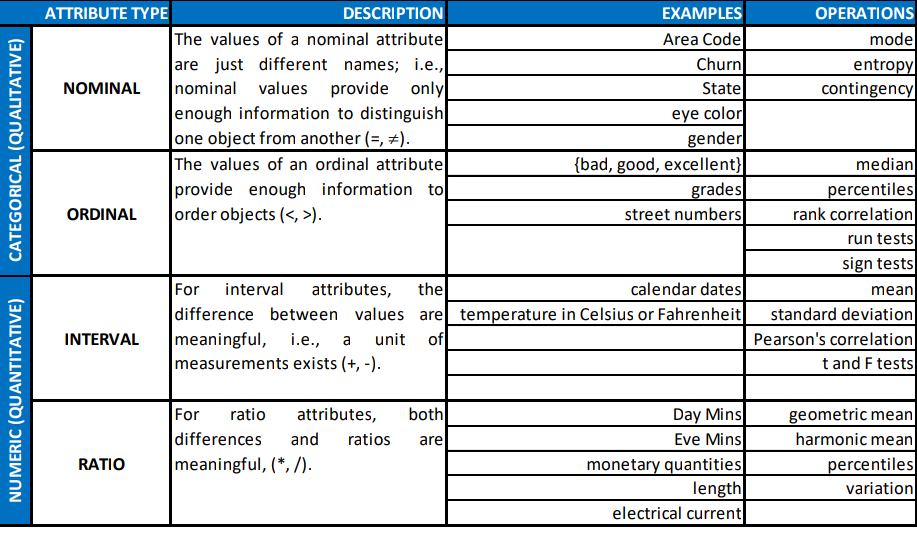
\includegraphics[height=0.5 \linewidth]{introduction/pict/attributi.png}
	\caption{Distinzione degli attributi con le relative proprietà}
\end{figure}
Dall'alto al basso il livello gerarchico sale e le proprietà aumentano.

C'è un'ulteriore divisione che può essere fatta ed è quella in:
Si possono anche dividere in attributi \textit{discreti} che possono essere:
\begin{itemize}
	\item Discreti (in cui la serie dei valori è finita o una infinità numerabile), che a loro volta si suddividono in:
	\begin{itemize}
		\item Categorici
		\item Numerici
		\item Binari: sono i più particolari da trattare, e hanno una serie di proprietà strane.
	\end{itemize}
	\item Continui, i cui valori sono numeri reali.
\end{itemize}

\subsection{Data exploration}

Dobbiamo però anche sapere come esplorare i dati in modo intelligente usando tutti i nostri strumenti a nostra disposizione. Diamo ora un elenco degli strumenti statistici più utili che ci permetton di avere un'analisi completa dei dati.

\subsubsection{Definizioni}
\begin{defn}
	Si definisce \textbf{quantile} $\alpha$ il valore $q_{\alpha}$ che divide la popolazione in due parti proporzionali rispettivamente ad $\alpha$ e a $(1 - \alpha)$ e caratterizzate da valori rispettivamente minori e maggiori di $q_{\alpha}$
\end{defn}

Un quantile molto importante è il quantile di ordine $\frac{1}{2}$ e si chiama \textbf{mediana} che è quello che ha esattamente minori di lui  metà dei dati.

\begin{defn}
	Si definisce \textbf{media} il seguente valore:
	\[mean = \frac{1}{n}\sum_{i=1}^{n}x_i\]
\end{defn}


La media non è un buon modo di visualizzare i dati perché dice poco riguardo alla loro distribuzione. Siccome la media è basata su singole osservazioni è fortemente soggetta a variazioni quando si hanno valori fortemente discostati dalla distribuzione dei dati.
Tali valori si chiamano \textit{outlier} e sono particolarmente interessanti da trattare.

Per ovviare a questo problema si è soliti usare  la \textbf{media trimmed} in cui si buttano via il valore più piccolo e il valore più grande. 
\begin{defn}
	Si definisce \textbf{media trimmed} il seguente valore:
	\[mean_{trimmed} = \frac{1}{n}\sum_{i=1}^{n}x_i  \qquad x_{i} = x - \max{x}- \min{x}\]
\end{defn}

Se si trova un grosso scostamento tra la media e la media trimmed probabilmente si ha la presenza di almeno un outlier.

\begin{defn}
	Si definisce \textbf{range} il seguente valore:
	\[ range = \max{x}- \min{x}\]
\end{defn}

Esso serve a quantificare la dispersione dei dati, ovviamente questo valore può essere fuorviante qualora i valori siano concentrati in una stretta banda di valori. Per ovviare a questo problema si usa la varianza.

\begin{defn}
	Si definisce \textbf{varianza} il seguente valore:
	\[ var =  \sigma^{2} =\frac{1}{n - 1 }\sum_{i = 1}^{n} (x_{i} - \bar{x})^{2}\]	
\end{defn}

E' preferibile però usare la deviazione standard in quanto per come è definita risulta essere della stessa unità di misura dei dati.
\begin{defn}
	Si definisce \textbf{deviazione standard} il seguente valore:
	\[ std = \sigma =  \sqrt{\sigma^{2}} \]
\end{defn}

Essendo queste due grandezze definite a partire dalla media esse soffrono dello stesso problema: sono fortemente condizionate dagli outlier, con lo stesso metodo precedente si definiscono quindi altre due grandezze in grado di ovviare a questo problema.

\begin{defn}
	Si definisce \textbf{deviazione media assoluta} il seguente valore:
	\[ AAD =  \frac{1}{n}\sum_{i=1}^{n}|x_i- mean|\]
\end{defn}

\begin{defn}
	Si definisce \textbf{deviazione mediana assoluta} il seguente valore:
	\[ MAD = mediana(x_{1}-mean, x_{2}-mean, ..., x_{n0}-mean )\]
\end{defn}

E' utile anche definire il range interquartile (IQR) sempre per ovviare alla presenza di outliar.

\begin{defn}
	Si definisce \textbf{deviazione mediana assoluta} il seguente valore:
	\[ IQR = q_{75\%} - q_{25\%}\]
\end{defn}

Ci sono anche diverse grandezze utili da definire nei casi in cui si ha a che fare con copppie di attributi, in tal caso:

\begin{defn}
	Si definisce \textbf{covarianza} il seguente valore:
\[cov(X,Y) = \frac{1}{m -1}\sum_{i = 1}^{m} (x_{i} - \bar{x})(y_{i} - \bar{y})\]
\end{defn}

Per come è costruita questa matrice è necessariamente quadrata, e il suo valore $ij ^{th}$ rappresenta la covarianza tra il valore $i^{th}$ dell'attributo x e il valore $j^{th}$ dell'attributo y.

Un'ulteriore misura dell'associazione tra le coppie di attributi quantitativi che non dipende dalla varianza di ciascun attributo è la seguente:

\begin{defn}
	Si definisce \textbf{correlazione di Pearson} il seguente valore:
	\[ corr(x,y) = \frac{cov(x,y)}{\sqrt{var(x)var(y)}}\]
\end{defn} 
Per come è definita si ha ovviamente che: $cov(x,y) \in [-1,1]$.

E' molto utile visualizzare i dati quando bisogna lavorarci, questo fondamentalmente per due motivi:
\begin{itemize}
	\item Ci permette di trovare pattern tra le variabili che valori puntuali non ci permetterebbero di trovare.
	\item Ci permette di visualizzare i risultati di una lavorazione fatta sui dati.
\end{itemize}

Di seguito proponiamo un rapido elenco dei grafici più utili e descriviamone le varie caratteristiche.

\subsubsection{Visualization}

Possono organizzare i dati in istogrammi caratterizzati dalla presenza di bin: essi indicano la larghezza in cui i dati sono organizzati. A seconda dell'ampiezza che uso posso ottenere due disegni molto diversi come mostrato in figura.


\begin{figure}[H]
	\centering
	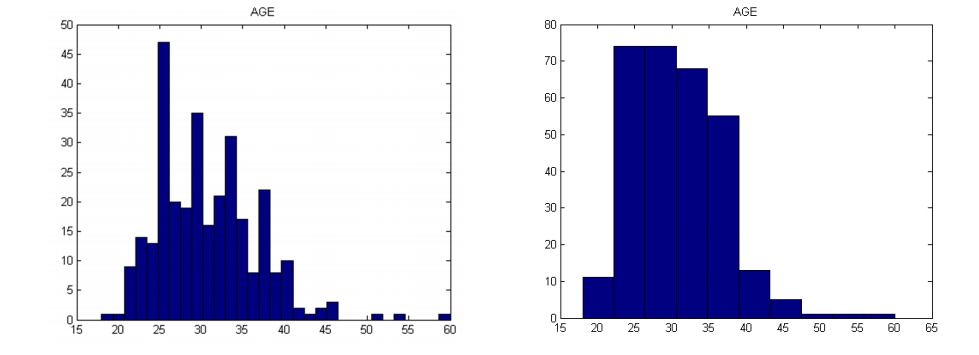
\includegraphics[height=0.35 \linewidth]{introduction/pict/istogramma_quant.png}
	\caption{Differenza tra due istogrammi fatti sulla stessa distribuzione di dati ma con numero di bin diversi.}
\end{figure}


Si possono allo stesso modo creare istogrammi per dati qualitativi. La differenza rispetto agli istogrammi sui dati quantitativi è quella per cui ogni bin corrisponde ad una categoria diversa.

\begin{figure}[H]
	\centering
	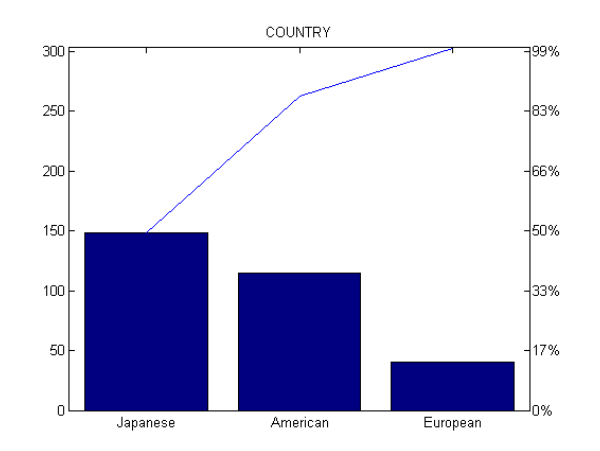
\includegraphics[height=0.3 \linewidth]{introduction/pict/istogramma_qual.png}
	\caption{Istogramma di dati qualitativi.}
\end{figure}

In questo caso la linea blu disegnata sopra è una linea cumulativa, ossia rappresenta dove si trova il livello sommando tutti i dati che man mano incontro, per come è costruita ovviamente dovrà finire sul valore $100\%$


Un altro modo di rappresentare i dati particolarmente utile è il \textbf{grafico Box and Whiskers} applicato solo ad attributi quantitativi. Rispetto agli istogrammi questo è decisamente più utilizzato perché permette di estrarre decisamente più informazioni. In particolare proponiamo un grafico in cui sono esplicitate le informazioni ottenibili:

\begin{figure}[H]
	\centering
	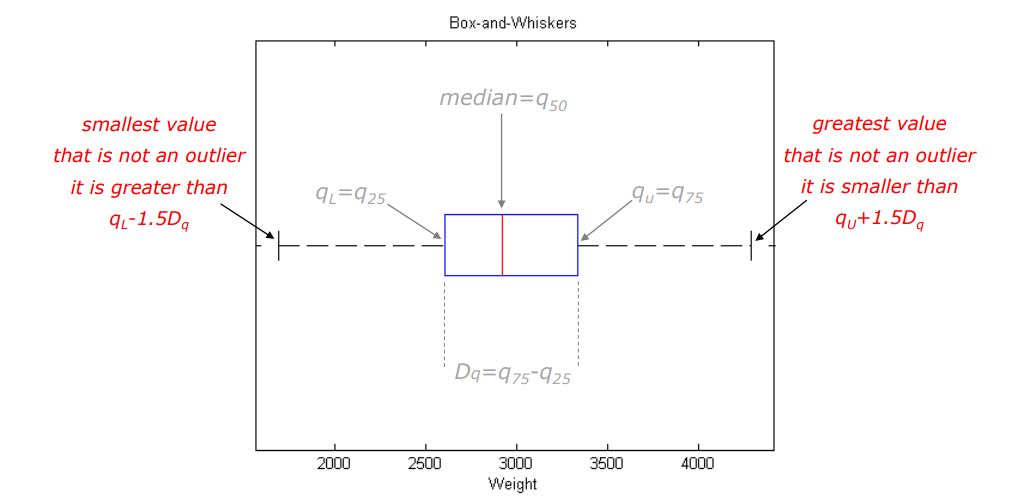
\includegraphics[height=0.4 \linewidth]{introduction/pict/box_plot.png}
	\caption{Informazioni ottenibili da un box plot.}
\end{figure}


\subsection{Missing replacement}

E' un problema enorme di per sè. Le operazioni più elementari sono le seguenti. In alcuni valori degli attributi un valore non è registrato. Ci possono esser tante ragioni: ad esempio un attributo non è sempre stato osservabile (penso all'ambito clinico), o ad esempio un attributo prima non veniva considerato rilevante.

Il primo nmetodo è il \textbf{Record removal} che è molto drastico come metodo perché comunque sia vengono eliminati dei valori che sarebbero potuti essere molto importanti.

Il secondo metodo è quello di \textbf{imputazione manuale}: è fatta da umani e tramite osservazioni ci si chiede se sia possibile inserirlo, è tremendamente difficile dal punto di vista computazionale.

Il terzo metodo è quello della \textbf{global constant}: ossia metto un numero là chiamato place holder con un valore costante, non troppo efficiente.

Il quarto metodo è quello di \textbf{rimpiazzarlo con la moda}, anche questo però è fortemente criticabile.
Se gli attributi sono continui si fa la stessa cosa ma con la media.

Il quinto metodo è \textbf{Conditional mean replacement} ossia bisogna rimpiazzare con la media solo se è presente un altro determinato attributo.

Il sesto metodo è quello del \textbf{most probable} ossia di prendere un modello e sostituire il valore.

E' molto difficile dare il confine tra l'esplorazione dei dati e la modellizzazione dei dati.

\subsection{Data Preprocessing}

Tutti questi processi impattano fortemente tutta l'analisi che farò dopo.



